% Lead: Colin? Eli? Yusra?
% Performance of the algorithms and known issues as seen in the data products
% Explain any residual artefacts DP1 data products that scientists shuld be aware of when doing sciene with DP1.
\section{Performance Characterization and Known Issues
\label{sec:performance}}
%
In this section, we provide an assessment of the \gls{DP1}
data quality and known issues.
A summary of the Rubin \gls{DP1} key numbers and data quality metrics  is found in PERFSUMMARYTABLE
%%%%%% This table is auto generated from data, DO NOT EDIT
\startlongtable
\begin{deluxetable*}{llcccccccc}
\caption{Rubin Observatory Data Preview 1 Key Numbers \label{tab:dp1_key_numbers}}
% \tablecolumns{8}
% \tablenum{1}
% \tablewidth{0pt}
% %\tabletypesize{\scriptsize}
\tablehead{
    \colhead{head1} &
    \colhead{head2} &
    \colhead{fdsafdsa} &
    \colhead{fdsafdsa} &
    \colhead{fdsafdsa} &
    \colhead{fdsafds} &
    \colhead{fdsafds} &
    \colhead{}
}
\startdata
    432432 & 32432432 & 43243243 & 432  & 432432  & 543232  & 54332  & 5432543 \\
\enddata
\end{deluxetable*}


\subsection{Sensor Anomalies and ISR}
\label{ssec:sensor_anomalies}
In addition to the known detector features identified before LSSTComCam commissioning, most of which are handled by the ISR processing (see \secref{ssec:isr}), we discovered a number of new types of anomalies in the DP1 data. 
Since no corrections are currently available for these anomalies, they are masked and excluded from downstream data products.

\subsubsection{Vampire Pixels}
Vampire pixels are visible on the images as a bright defect surrounded by a region of depressed flux, as though the defect is stealing charge from its neighboring pixels; they have been termed ``vampire'' defects.
 \figref{fig:anomalies_vampire_pixels}  shows an example of a vampire pixel near the center of R22\_S11 on an r-band flat.

From studies on evenly illuminated images, vampires appear to conserve charge.
Unfortunately, there's no clean way to redistribute this stolen flux, and so we have identified as many of them as possible and created manual defect masks to exclude them from processing.
We have found some similar features on the ITL detectors on LSSTCam, and will use the same approach to exclude them.
\begin{figure}[htb!]
  \centering
  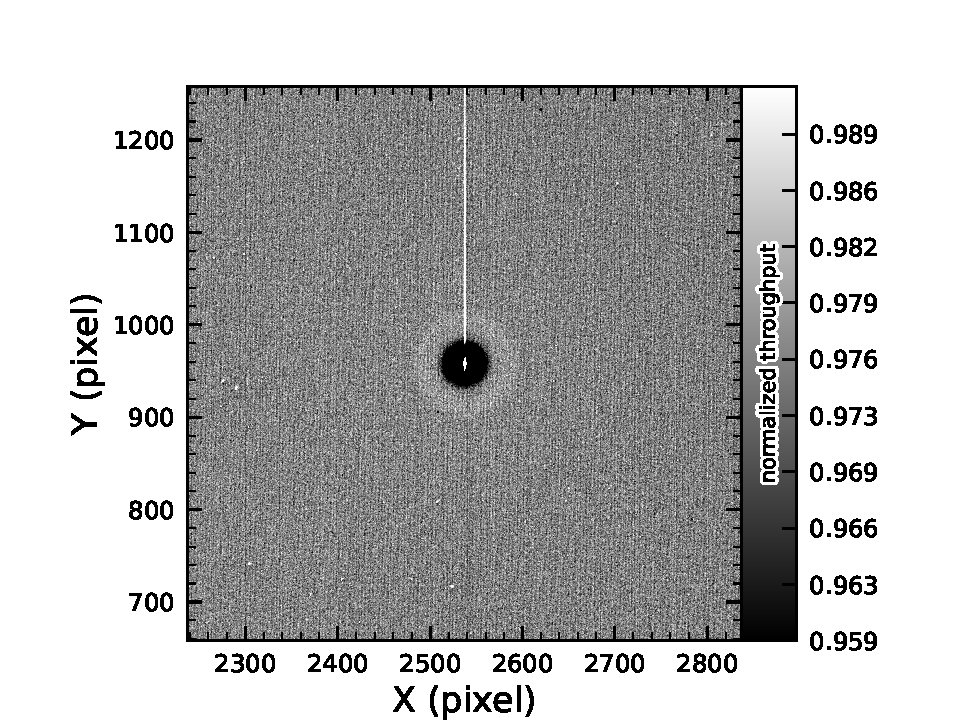
\includegraphics[width=0.98\linewidth]{figures/dp1_isr_anomalies-vampire_pixel.pdf}
  \caption{A large \textit{vampire pixel} near the center of R22\_S11, as seen on the r-band flat.}
   \label{fig:anomalies_vampire_pixels}
\end{figure}

\subsubsection{Phosphorescence}
Some regions were seen to contain large numbers of bright defects.
An example is shown in   \figref{fig:anomalies_phosphorescence}  in a g-band flat. 
On closer study, it appears that on some detectors a layer of photoresist wax was incompletely removed from the detector surface during production.
As this wax is now trapped below the surface coatings, there is no way to physically clean these surfaces.
If this wax responded to all wavelengths equally, then it would likely result in quantum efficiency dips, which might be removable during flat correction.
However, it appears that this wax is slightly phosphorescent, with a decay time on the order of minutes, resulting in the brightness of these sources being dependent on the illumination of prior exposures.
The worst of these regions were excluded with manual masks, but we do not expect to need to do this for LSSTCam.
\begin{figure}[htb!]
  \centering
  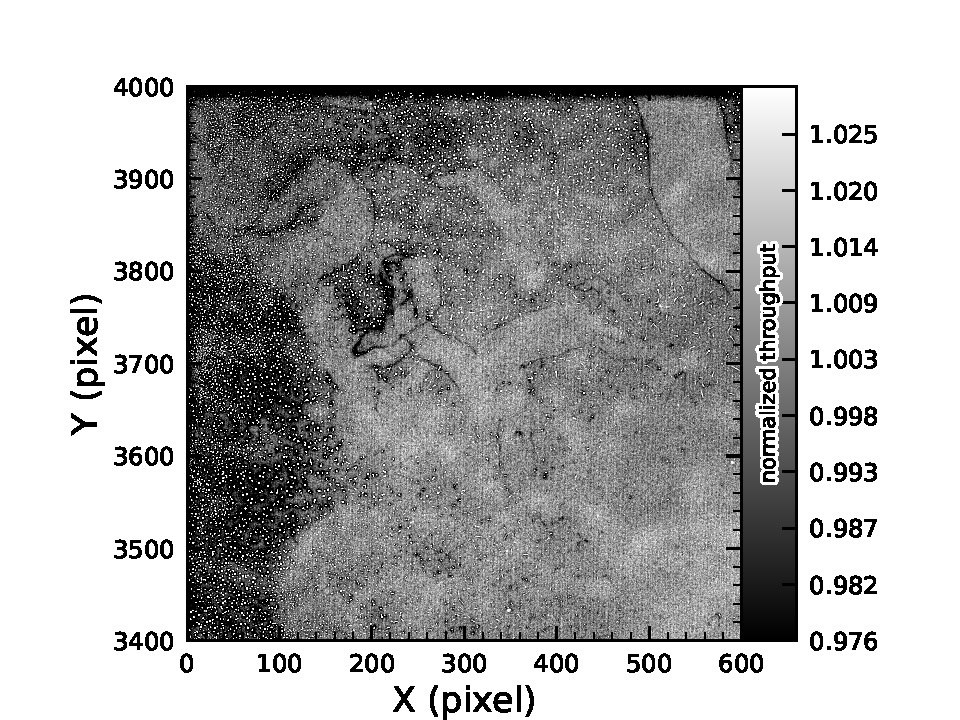
\includegraphics[width=0.98\linewidth]{figures/dp1_isr_anomalies-phosphorescence.pdf}
  \caption{The top left corner of R22\_S01 in the g-band flat, showing the many small defect features that are caused by the remnant photoresist wax.
  A single large defect box masks this region from further analysis to prevent these features from contaminating measurements.}
  \label{fig:anomalies_phosphorescence}
\end{figure}

\subsubsection{Crosstalk}
We use an average crosstalk correction based on laboratory measurements with LSSTCam.
These average corrections performed better than expected, and so have been used as-is for DP1 processing.
There are, however, some residual crosstalk features present post-correction, with a tendency towards over-subtraction.
\figref{fig:crosstalk_residual} shows an example  of a bright star with over-subtracted crosstalk residuals visible on neighboring amplifiers to both sides on exposure 2024120600239, detector R22\_S02.
\begin{figure}[htb!]
  \centering
  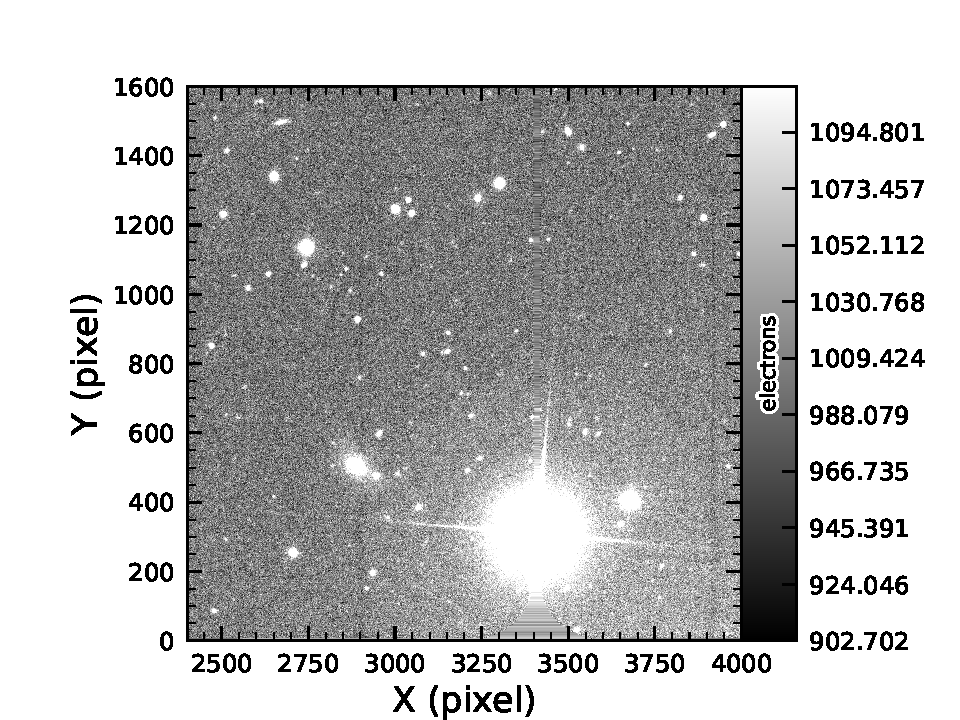
\includegraphics[width=0.98\linewidth]{figures/dp1_isr_anomalies-crosstalk_residual.pdf}
  \caption{An example of a bright star with over-subtracted crosstalk residuals visible on neighboring amplifiers to both sides (exposure 2024120600239, detector R22\_S02).
  The horizontal banding stretching from the center of the star shows the interpolation pattern covering the saturated core and the ITL edge bleed near the serial register.}
  \label{fig:crosstalk_residual}
\end{figure}

\subsubsection{Bleed Trails}
Bleed trails from saturated sources were expected on LSSTComCam, but they appear in more dramatic forms than was expected.
As a bleed trail nears the serial register, it fans out into a ``trumpet'' shaped feature.
Although bright, these features do not have consistently saturated pixels.
In DP1 these ``edge bleeds'' were programmatically identified and masked.

Saturated sources can create a second type of bleed, where the central bleed drops below the background level.
The depressed columns along these trails extend across the entire height of the detector, crossing the detector mid-line.
We developed a model for these to identify which sources are sufficiently saturated to result in such a trail, which is then masked.  As these kind of trails appear only on the ITL detectors, we've named these features ``ITL dips.''
\figref{fig:anomalies_itl_dip} shows an example of a   bright star exhibiting the ``ITL dip'' phenomenon on exposure: 2024121000503, detector: R22\_S21.
\begin{figure}[htb!]
  \centering
  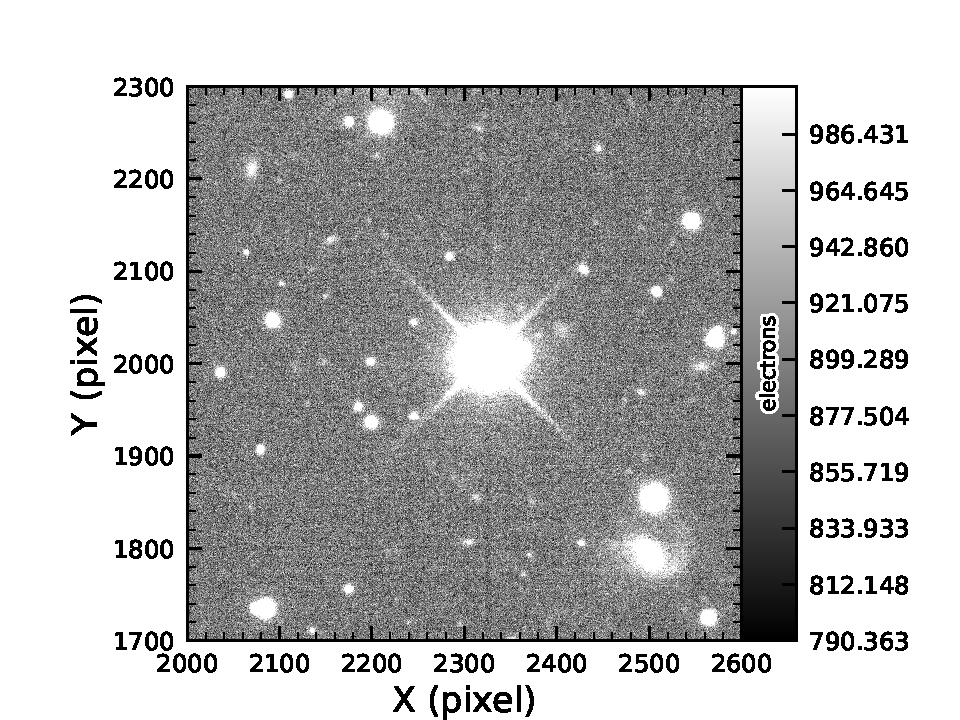
\includegraphics[width=0.98\linewidth]{figures/dp1_isr_anomalies-itl_dip.pdf}
  \caption{A bright star showing the ``ITL dip'' phenomenon, in which a dark trail extends out from the star to the top and bottom edges of the detector (exposure: 2024121000503, detector: R22\_S21).}
\label{fig:anomalies_itl_dip}
\end{figure}


% Pierre-François
\subsection{PSF Models
\label{ssec:psf_models}}

To characterize \gls{PSF} performance, we use adaptive second moments (\citealt{2002AJ....123..583B})
measured on \gls{PSF} stars and on the PSF model using the \gls{HSM} 
implementation (\citealt{2003MNRAS.343..459H} and \citealt{2005MNRAS.361.1287M}), 
all expressed in each detector's pixel frame.
We consider the classical trace of the second moment matrix $T$, along with the ellipticity parameters $e^1$ and $e^2$, to characterize the performance of the PSF.
We denote $T_{\text{PSF}}$, $e^1_{\text{PSF}}$, and $e^2_{\text{PSF}}$ for
measurements on the \gls{PSF} stars, and $T_{\text{model}}$, $e^1_{\text{model}}$,
and $e^2_{\text{model}}$ for the \gls{PSF} model. Two variants are compared:
\begin{itemize}
\item Piff with second-order polynomial interpolation (default in science pipelines); and
\item Piff with fourth-order polynomial interpolation (final \gls{DP1} \gls{PSF}).
\end{itemize}

Table \ref{tab:psf-1d_stats} summarizes each model’s ability to reconstruct
the mean $T$, $e^1$, and $e^2$ on  \gls{LSSTComCam}. Piff shows a negative
residual bias in size. 
\begin{deluxetable*}{lccc}
\caption{Comparison of observed and model residuals, across all visits and filters.}
\label{tab:psf-1d_stats}
\tablehead{
  \colhead{\textbf{Quantity}} & 
  \colhead{\textbf{Observed}} & 
  \colhead{\textbf{Piff O2}} & 
  \colhead{\textbf{Piff O4}} \\
  \colhead{} & 
  \colhead{} & 
  \colhead{$\times10^{-4}$} & 
  \colhead{$\times10^{-4}$} 
}
\startdata
$\langle T\rangle\ (\mathrm{pixel}^2)$ & $11.366 \pm 0.003$ & & \\
$\langle e^1\rangle$ & $(-6.07\pm0.05)\times10^{-3}$ & & \\
$\langle e^2\rangle$ & $(-4.57\pm0.05)\times10^{-3}$ & & \\
$\langle e\rangle$ & $(8.794\pm0.004)\times10^{-2}$ & & \\
$\langle \delta T / T\rangle$  & & $-4.0\pm0.2$ & $-5.0\pm0.2$ \\
$\langle \delta e^1\rangle$ & & $0.6\pm0.1$ & $0.5\pm0.1$ \\
$\langle \delta e^2\rangle$ & & $0.0\pm0.1$ & $0.0\pm0.1$ \\
\enddata
\end{deluxetable*}

% \begin{table}[ht]
%   \centering
%   \caption{Comparison of observed and model residuals, across all visits and filters.}
%   \label{tab:psf-1d_stats}
%   \begin{tabular}{l c c c}
%     \toprule
%     & Observed 
%     & Piff (order 2) 
%     & Piff (order 4) \\
%     \midrule
%     $\langle T\rangle\ (\mathrm{pixel}^2)$ 
%       & $11.366 \pm 0.003$ 
%       & 
%       & 
%     \\[4pt]
%     $\langle e^1\rangle$ 
%       & $(-6.07\pm0.05)\times10^{-3}$ 
%       & 
%       & 
%     \\[4pt]
%     $\langle e^2\rangle$ 
%       & $(-4.57\pm0.05)\times10^{-3}$ 
%       & 
%       & 
%     \\[4pt]
%     $\langle e\rangle$ 
%       & $(8.794\pm0.004)\times10^{-2}$
%       & 
%       & 
%     \\[8pt]
%     $\langle \delta T / T\rangle$ 
%       & 
%       & $(-4.0\pm0.2)\times10^{-4}$ 
%       & $(-5.0\pm0.2)\times10^{-4}$
%     \\[4pt]
%     $\langle \delta e^1\rangle$ 
%       & 
%       & $(0.6\pm0.1)\times10^{-4}$ 
%       & $(0.5\pm0.1)\times10^{-4}$
%     \\[4pt]
%     $\langle \delta e^2\rangle$ 
%       & 
%       & $(0.0\pm0.1)\times10^{-4}$ 
%       & $(0.0\pm0.1)\times10^{-4}$
%     \\
%     \bottomrule
%   \end{tabular}
% \end{table}

Another way to assess \gls{PSF} performance is to examine the average
across visits of $\delta T/T$ projected onto focal-plane coordinates
(\figref{fig:psf_residuals_fov}).
Piff shows strong spatial correlations, with a systematic offset
that matches Table \ref{tab:psf-1d_stats}. It is the existence of these spatial structures that motivated raising the interpolation order to four, except in the u-band.
Although not shown in \figref{fig:psf_residuals_fov}, third-order polynomial interpolation still exhibited residual structure.
A fifth-order polynomial interpolation would require more stars than are available on some CCDs to adequately constrain the model while offering only marginal gains.
Preliminary analysis of LSSTCam data in the laboratory at \gls{SLAC} shows that the \gls{ITL} sensors exhibit the same pattern as \gls{ITL} sensors on \gls{LSSTComCam}.
The sensor's $\delta T/T$ is fully correlated with the height variation across the LSSTCam \gls{ITL} sensors, which explains this behavior.
Future data processing will account for this height variation directly in the \gls{PSF} model.
\begin{figure}[htb!]
\centering
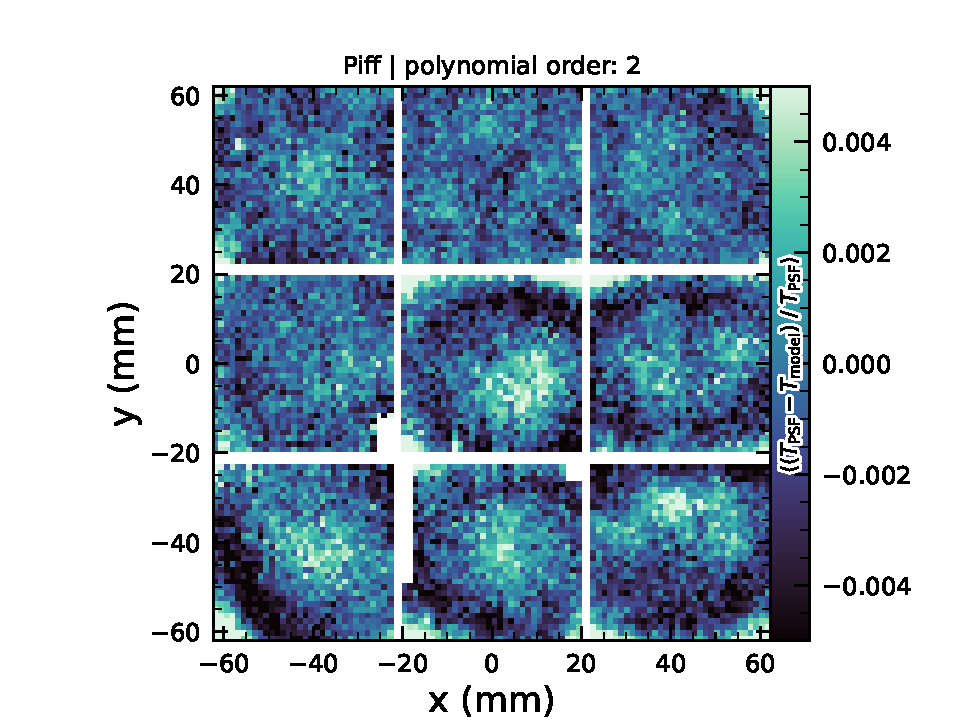
\includegraphics[scale=0.29]{figures/dT_T_Piff_poly_order_2.pdf}
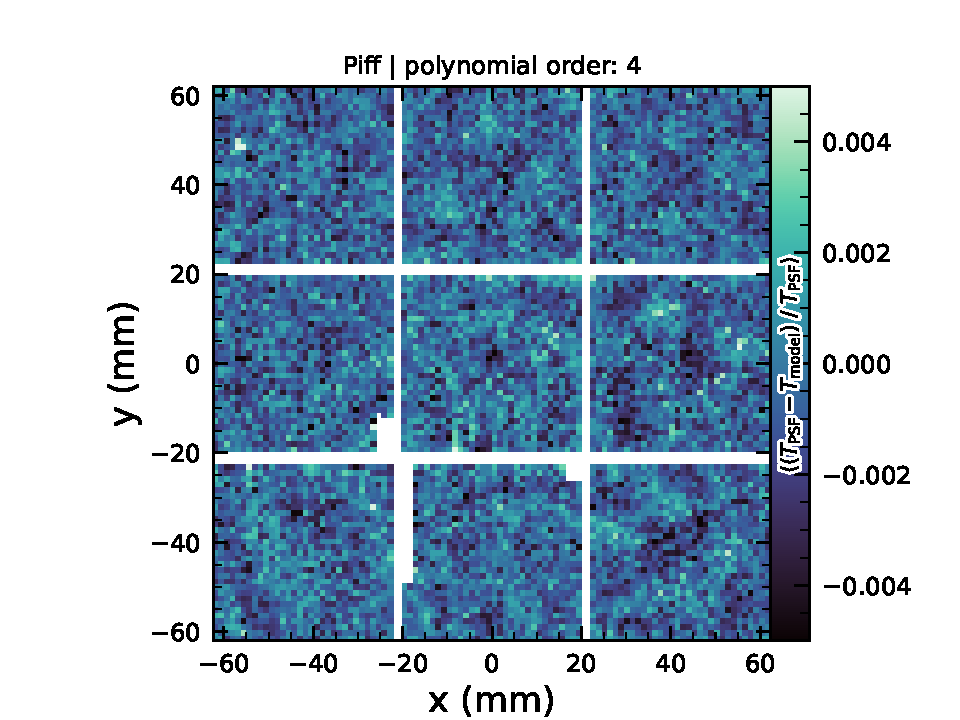
\includegraphics[scale=0.29]{figures/dT_T_Piff_poly_order_4.pdf}
\caption{\small Average across all visits of $\delta T/T$  for different PSF modeling on \gls{LSSTComCam}. Average is computed on a bin size of 120 pixels.}
\label{fig:psf_residuals_fov}
\end{figure}

Another way to look at the \gls{PSF} modeling quality is via whisker plots of the \gls{PSF} second and fourth moments and their modeling residuals projected on a part of the sky.
In addition to the second moment, the spin-2 fourth moments, $e^{(4)}$, are defined as:
\begin{align*}
e^{(4)}_1 &= M_{\text{40}} - M_{\text{04}} \\
e^{(4)}_2 &= 2\left(M_{\text{31}} - M_{\text{13}}\right),
\end{align*}
where $M_{\text{pq}}$ are the standardized higher moments as defined in \cite{2023MNRAS.520.2328Z} measured on stars and PSF models.
Figure \ref{fig:psf_residuals_whisker_ECDFS} shows
the whisker plots of $e$, $e^{(4)}$ (top rows), and $\delta e$, $\delta e^{(4)}$
in the \gls{ECDFS} field. The direction of the whiskers represents the orientation of the \gls{shape}, while the length, modulated by the red bar, represents the amplitude $|e|$ or $|e^{(4)}|$.
We observe coherent patterns in both the \gls{PSF} moments and the residuals, the latter of which warrants further investigation if it persists in future data releases.
\begin{figure}[htb!]
    \centering
    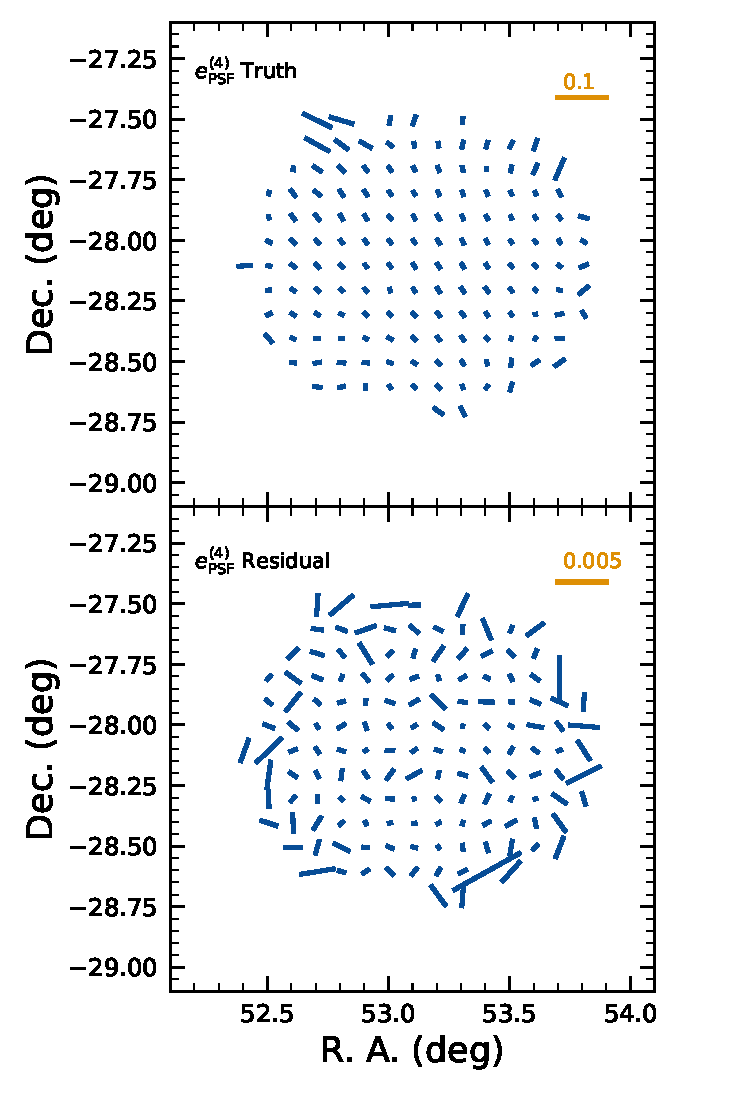
\includegraphics[scale=0.33]{figures/performance/psf_fourth_whisker.pdf}
    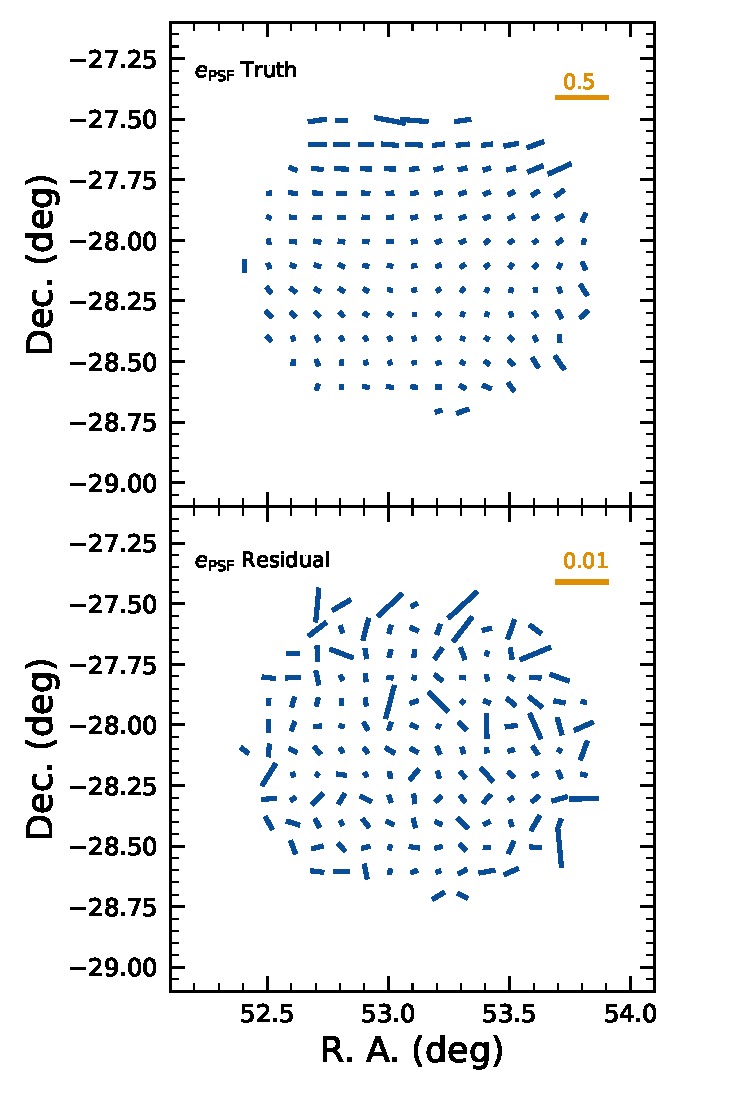
\includegraphics[scale=0.33]{figures/performance/psf_second_whisker.pdf}
    \caption{\small Whisker plot on \gls{ECDFS} field for $e$, $e^{(4)}$ and $\delta e$, $\delta e^{(4)}$.}
    \label{fig:psf_residuals_whisker_ECDFS}
\end{figure}

Another characterization of \gls{PSF}-modeling performance is to look at $\delta T/T$ versus stellar magnitude to reveal any \gls{PSF} size–flux dependencies (\figref{fig:psf_residuals_mag_color}). 
We also repeat this analysis in color bins to probe chromatic effects. 
Fainter stars show a larger negative bias in \gls{PSF} size compared to brighter ones. 
Binning by color uncovers a clear color dependence, as seen in \gls{DES} (e.g., \citealt{DES:2020vau}). 
DP1 does not include the color correction implemented in \cite{2025OJAp....8E..26S}.
Post-DP1 tests added a color correction similar to \cite{2025OJAp....8E..26S}: it reduced the color-dependent scatter in PSF size but did not eliminate the negative bias for faint sources.
The cause of this residual remains unknown and is consistent with what is shown in Table \ref{tab:psf-1d_stats}.

\begin{figure}[htb!]
\centering
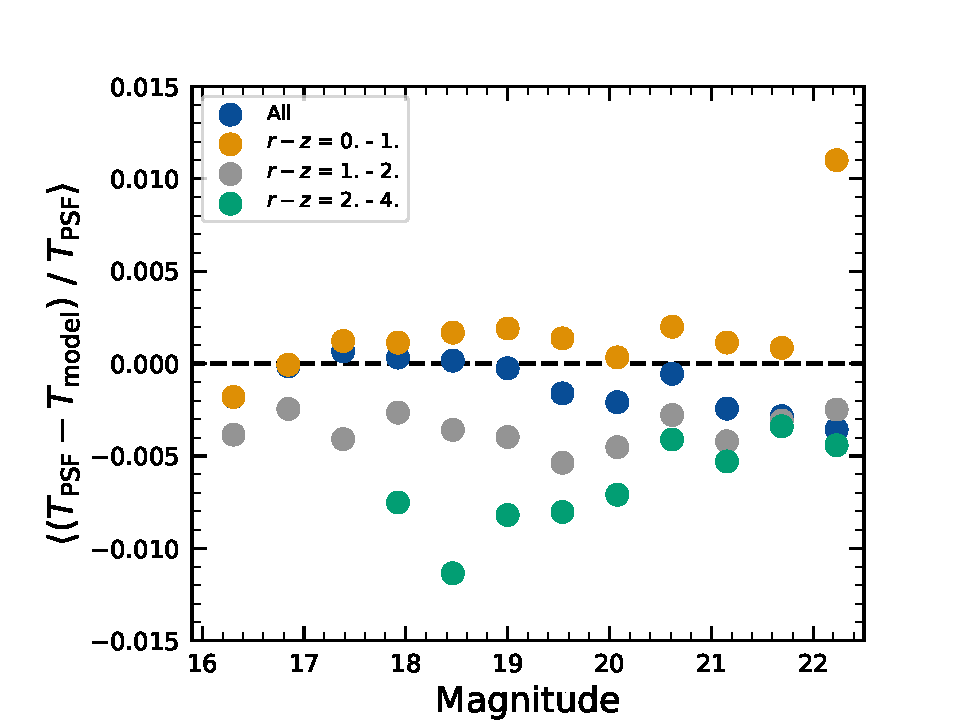
\includegraphics[width=0.98\linewidth]{dT_T_Piff_poly_4_vs_mag.pdf}
\caption{Binned $\delta T/T$ as a function of magnitude across
all visits and filters and binned in different colors.}
\label{fig:psf_residuals_mag_color}
\vspace{0.1cm}
\end{figure}

As noted in  \cite{PSTN-019}, two key Piff features were not used in the DP1 processing. 
PSF color dependence wasn’t implemented, and, while Rubin software allows Piff to work with sky coordinates (including WCS transformations), it doesn’t yet correct for sensor-induced astrometric distortions such as tree rings. 
Both features are planned for upcoming releases.


% Clare or Pierre-François
\subsection{Astrometry}
%Technotes referenced in https://rubinobs.atlassian.net/browse/DM-9040
%Reference Frame and epoch, WCS
To characterize astrometric performance, we evaluate both internal consistency and agreement with an external reference.
A primary measure of internal consistency is the repeatability of position measurements for the same object. We associate isolated point sources across visits and compute the \gls{RMS} of their fitted positions.
\figref{fig:AM1_and_dm_astro_error} shows the median per-\gls{tract} astrometric error for all isolated point sources, both after the initial calibration and after the final calibration, which includes proper motion corrections.
The results indicate that the astrometric solution is already very good after the initial \gls{calibration}.
Global calibration yields only modest improvement, likely due to the short time span of \gls{DP1} and the minimal distortions in the LSSTComCam.
In the main survey, the longer time baseline and greater distortions near the \gls{LSSTCam} field edges will make global calibration more impactful.
% \begin{figure}[htb!]
% \centering
% \includegraphics[width=0.98\linewidth]{Astrometry_dmAstroErr.pdf}
% \caption{Mean per-tract astrometric repeatability of measurements of isolated point sources in RA.}
% \label{fig:dmAstroErr}
% \end{figure}

An additional \gls{metric} of internal consistency is the repeatability of separations between objects at a given distance.
To calculate this, we find pairs of objects at a given distance from each other, then calculate their separation in each visit in which they appear.
The scatter in these distances then gives us a measure of the internal consistency of the astrometric model.
The median value for each tract for objects separated by approximately 5~arcmin after the final calibration, i.e., AM1 from \citet{LPM-17}, is given in \figref{fig:AM1_and_dm_astro_error}.
% \begin{figure}[htb!]
% \centering
% \includegraphics[width=0.98\linewidth]{Astrometry_AM1.pdf}
% \caption{Median per-tract repeatability in separations between isolated point sources 5~arcmin apart.}
% \label{fig:AM1}
% \vspace{0.1cm}
% \end{figure}
These values are already approaching the design requirement of $10$ mas.

\begin{figure}[htb!]
\centering
\includegraphics[scale=0.29]{figures/Astrometry_dmAstroErr.pdf}
\includegraphics[scale=0.29]{figures/Astrometry_AM1.pdf}
\caption{(a) Mean per-tract astrometric repeatability of measurements of isolated point sources in \gls{RA} (b) Median per-tract repeatability in separations
between isolated point sources 5 \gls{arcmin} apart.}
\label{fig:AM1_and_dm_astro_error}
\end{figure}

Finally, we consider the median separation between sources not included in the astrometric fit and associated objects from a reference catalog.
For this, we use the Gaia \gls{DR3} catalog, with the object positions shifted to the observation epoch using the Gaia proper motion parameters.
Figure~\ref{fig:AA1} shows the median separation for each visit in the r-band in \gls{tract} 4849.
\begin{figure}[htb!]
\centering
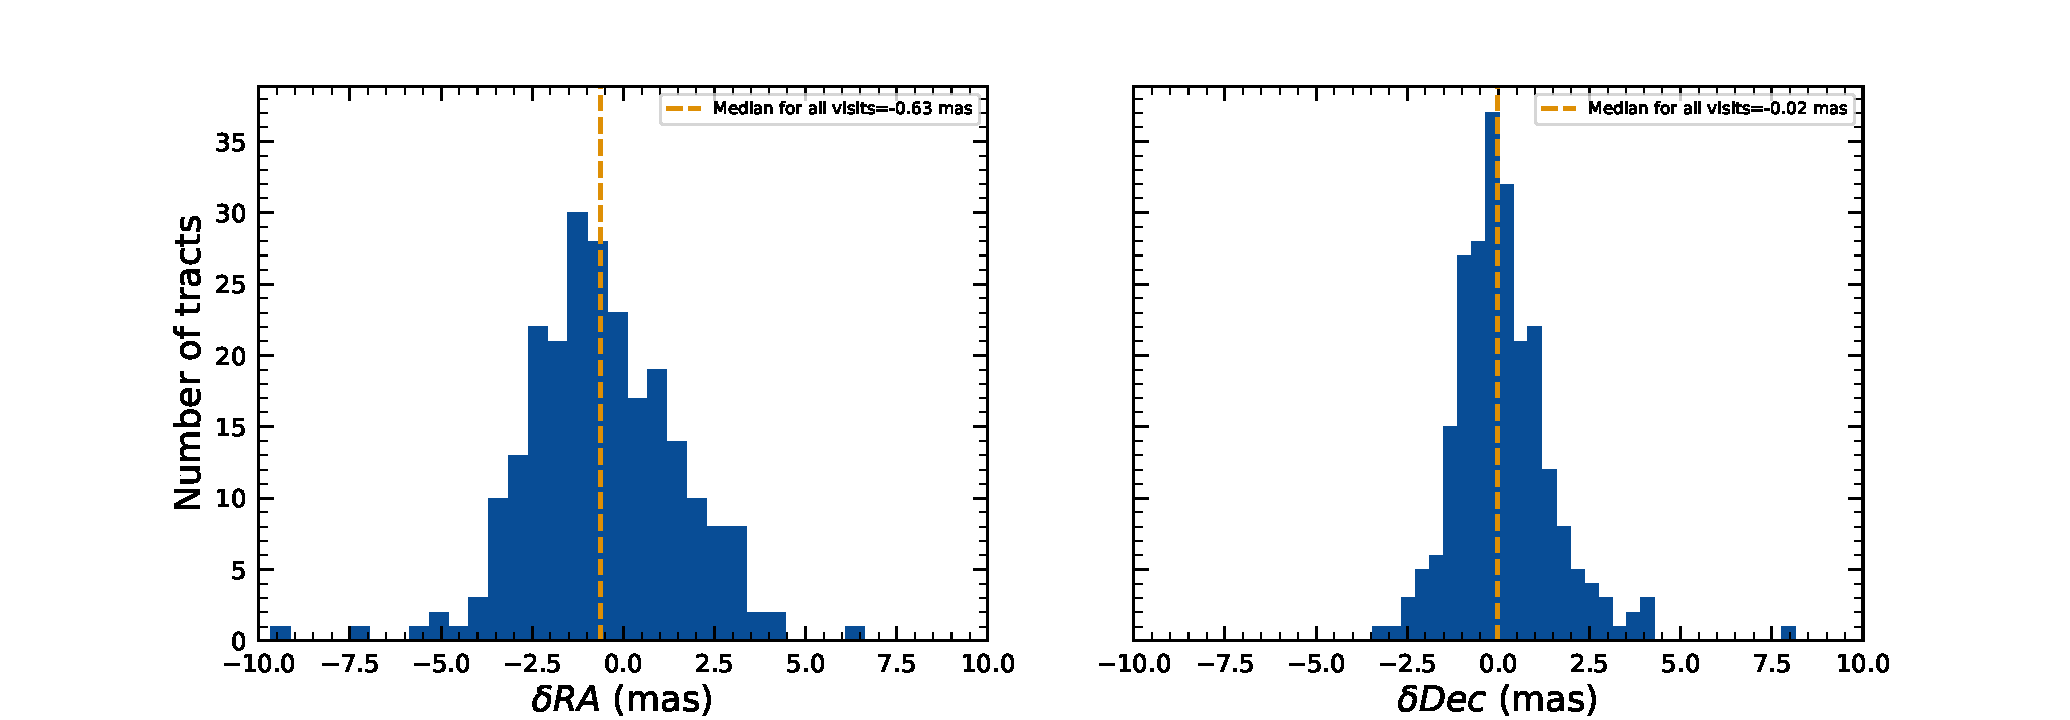
\includegraphics[width=0.98\linewidth]{Astrometry_AA1.pdf}
\caption{Median absolute offset for all visits in r-band in \gls{tract} 4849. The offset is the difference between the position of isolated point sources that were reserved from the astrometric fit and matched objects from the Gaia DR3 catalog.}
\label{fig:AA1}
\vspace{0.1cm}
\end{figure}


The calculated values are almost all within $5$\xspace mas, well below the design requirement of $50$\xspace mas for the main survey.

By looking at the astrometric residuals, we can assess whether there are distortions not accounted for by the astrometric model.
In some cases, the residuals in a single visit show behavior consistent with atmospheric turbulence, as shown in Figure~\ref{fig:Astrometry_Emode}.
As in \citet{Leget2021} and \citet{Fortino2021}, this is characterized by a curl-free gradient field in the two-point correlation function of the residuals (E-mode). However, as seen in Figure~\ref{fig:Astrometry_EBmode}, the residuals in many visits also have correlation functions with a non-negligible divergence free B-mode, indicating that some of the remaining residuals are due to unmodeled instrumental effects, such as rotations between visits.
\begin{figure*}[htb!]
\centering
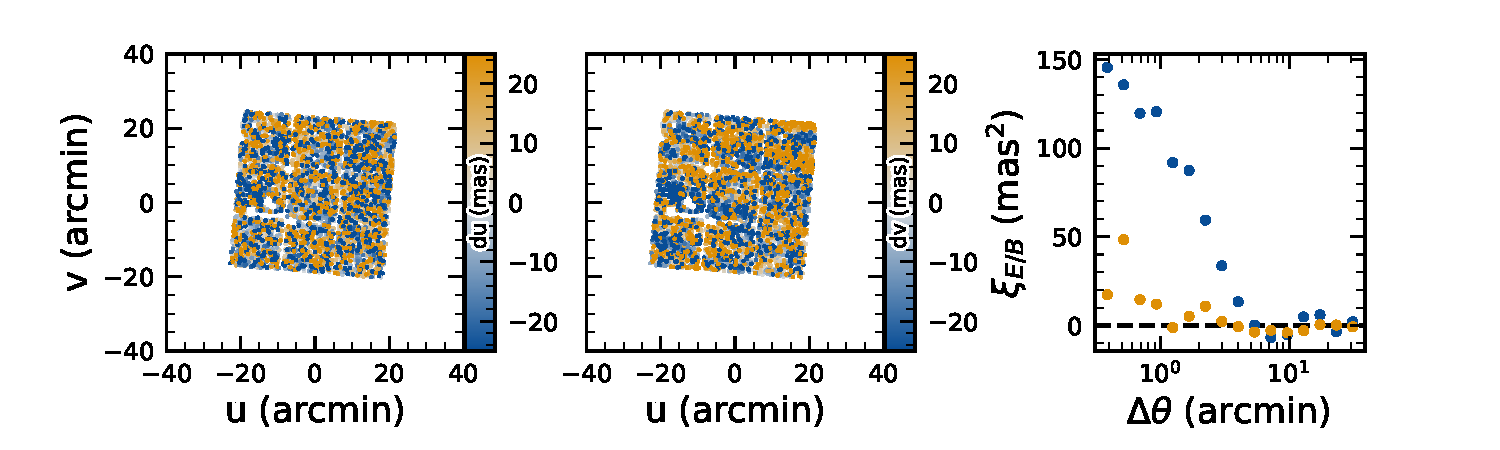
\includegraphics[width=0.98\linewidth]{figures/Astrometry_2024120200359.pdf}
\caption{\small Residuals in $du$ (left panel) and $dv$ (center panel) directions, with the E and \gls{B}-modes of the two-point correlation function (right panel). The residuals show a wave-like pattern characteristic of atmospheric turbulence, and there is significant E-mode and negligible \gls{B}-mode in the correlation function.}
\label{fig:Astrometry_Emode}
\vspace{0.1cm}
\end{figure*}


\begin{figure*}[htb!]
\centering
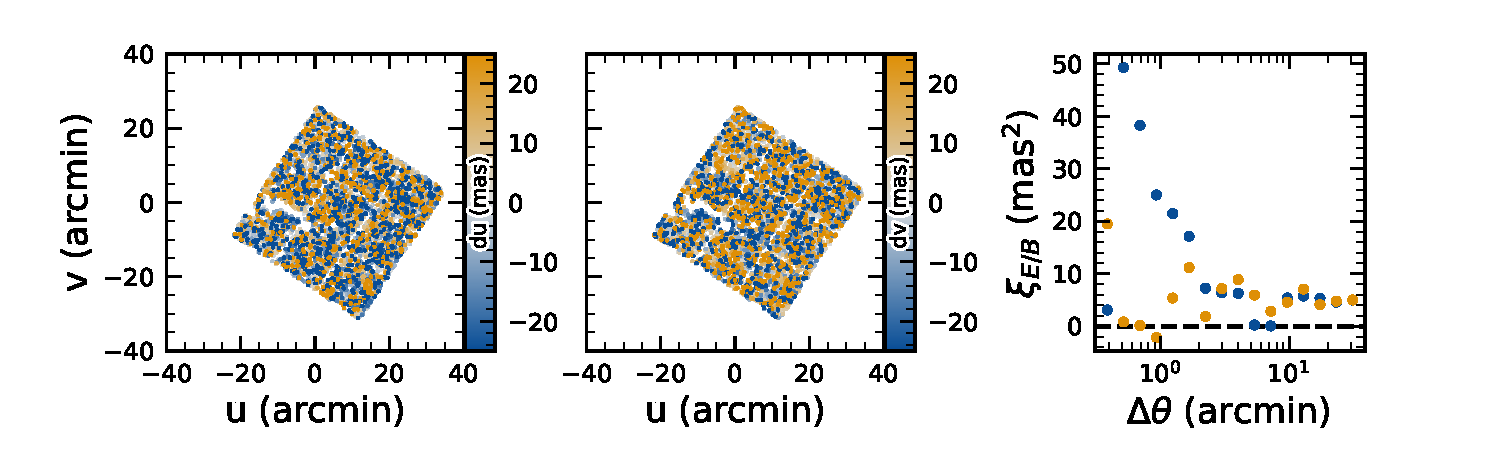
\includegraphics[width=0.98\linewidth]{Astrometry_2024120700527.pdf}
\caption{\small Residuals in $du$ (left panel) and $dv$ (center panel) directions, with the E and \gls{B}-modes of the two-point correlation function (right panel). There are coherent residuals, but without the wave-like patter seen in Figure~\ref{fig:Astrometry_Emode}, and the correlation function has significant values for both E and \gls{B}-modes.}
\label{fig:Astrometry_EBmode}
\vspace{0.1cm}
\end{figure*}

We can see unmodeled \gls{camera} distortions by stacking the residuals over many visits as a function of the focal plane position.
Figure~\ref{fig:Astrometry_FoV} shows the median residuals in x and y directions for \nvisits visits.
\begin{figure}[htb!]
\centering
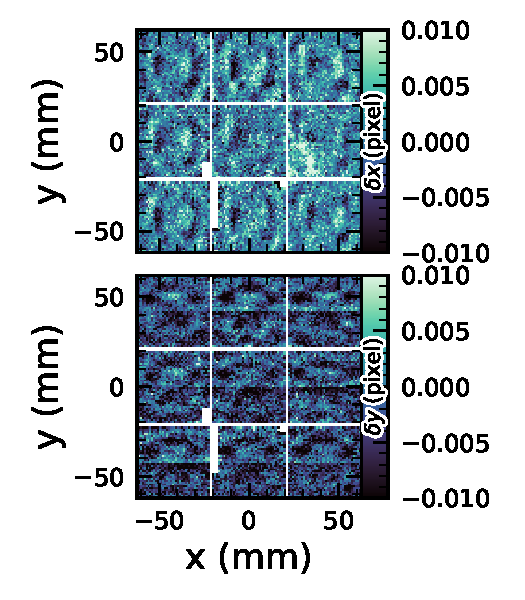
\includegraphics[width=\linewidth]{Astrometry_FoV.pdf}
\caption{Median residuals as a function of focal plane position in $dx$ (left panel) and $dy$ (right panel) directions}
\label{fig:Astrometry_FoV}
\end{figure}
Spatial structures are evident at the \gls{CCD} level, along with the mid-line break in the y-direction residuals.

Further stacking all the detectors makes certain effects particularly clear.
Figure~\ref{fig:Astrometry_CCD} shows distortions very similar to those measured for an \gls{LSSTCam} \gls{ITL} sensor in a laboratory setting in \citet{2023PASP..135k5003E}.
\begin{figure}[htb!]
\centering
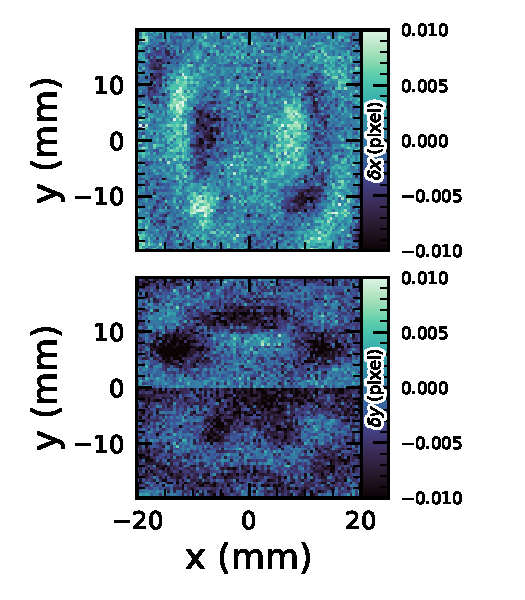
\includegraphics[width=1.0\linewidth]{Astrometry_CCD.pdf}
\caption{\small Median residuals as a function of pixel position in $dx$ (left panel) and $dy$ (right panel) directions}
\label{fig:Astrometry_CCD}
\end{figure}

\subsection{Photometry}

The photometric repeatability for isolated bright stars after the FGCM fits was excellent.
Across a broad range of colors, including chromatic corrections, the repeatability for the 10\% of stars reserved from the fit (signal-to-noise $> 100$) was $7.1/5.4/5.4/5.1/5.9/6.5\,mmag$ for $ugrizy$ respectively across all the fields.
Taking into account the photometric noise, the intrinsic repeatability was approximately
$4.8/2.7/1.7/1.0/2.0/1.1\,mmag$ for $ugrizy$ stars.
Our pipeline does not yet include chromatic corrections in the final photometry.
In this case the delivered photometric repeatability was $3-8\,mmag$ for grizy.

In \figref{fig:stellarloci}, we show the stellar loci for $ugriz$ from the full DP1 object table.
The narrow widths of these stellar loci show that our photometric performance is where we expect it to be given the nature of the LSSTComCam system.

\begin{figure*}[hbt!]
  \centering
  \begin{subfigure}[t]{0.31\textwidth}
  \includegraphics[width=\linewidth, height=5.8cm]{dp1_stellar_locus_ugr.pdf}
  \caption{$ugr$ stellar locus containing 12779 stars with signal-to-noise greater than 50 in the $u$ band.}
  \end{subfigure}\hfill
  \begin{subfigure}[t]{0.31\textwidth}
  \includegraphics[width=\linewidth, height=5.8cm]{dp1_stellar_locus_gri.pdf}
  \caption{$gri$ stellar locus containing 63236 stars with signal-to-noise greater than 200 in the $i$ band.}
  \end{subfigure}\hfill
    \begin{subfigure}[t]{0.31\textwidth}
  \includegraphics[width=\linewidth, height=5.8cm]{dp1_stellar_locus_riz.pdf}
  \caption{$riz$ stellar locus containing 46760 stars with signal-to-noise greater than 200 in the $i$ band.}
  \end{subfigure}\hfill
\caption{Examples of stellar loci from the full DP1 data set.}
  \label{fig:stellarloci}
\end{figure*}

%%
\subsection{Detection Completeness on Coadds}
\label{ssec:detection_completeness}
We characterize completeness by injecting synthetic sources into coadded images, and by comparing to external catalogs.
In both cases, we use a greedy, probabilistic matching \gls{algorithm}, whereby reference objects are matched in order of descending brightness to the most likely target within a $0.5''$ radius.

We inject sources in 12 of the patches of the \gls{ECDFS} region with the deepest coverage.
The input catalog contains stars and galaxies from part of the \gls{DC2} simulations \citep{2021ApJS..253...31L}, where the galaxies consist of an exponential disk and de Vaucouleurs \citep{1948AnAp...11..247D,1953MNRAS.113..134D} bulge.
To avoid deblender failures from excessive increases in object density, stars whose total \gls{flux} (i.e., summed across all six bands) is brighter than 17.5~${\rm mag_{\rm AB}}$ are excluded, as are galaxies whose total \gls{flux} is brighter than 15~${\rm mag_{AB}}$ or fainter than 26.5~${\rm mag_{AB}}$. Half of the remaining objects are selected for injection.

\begin{figure}[htb]
\centering
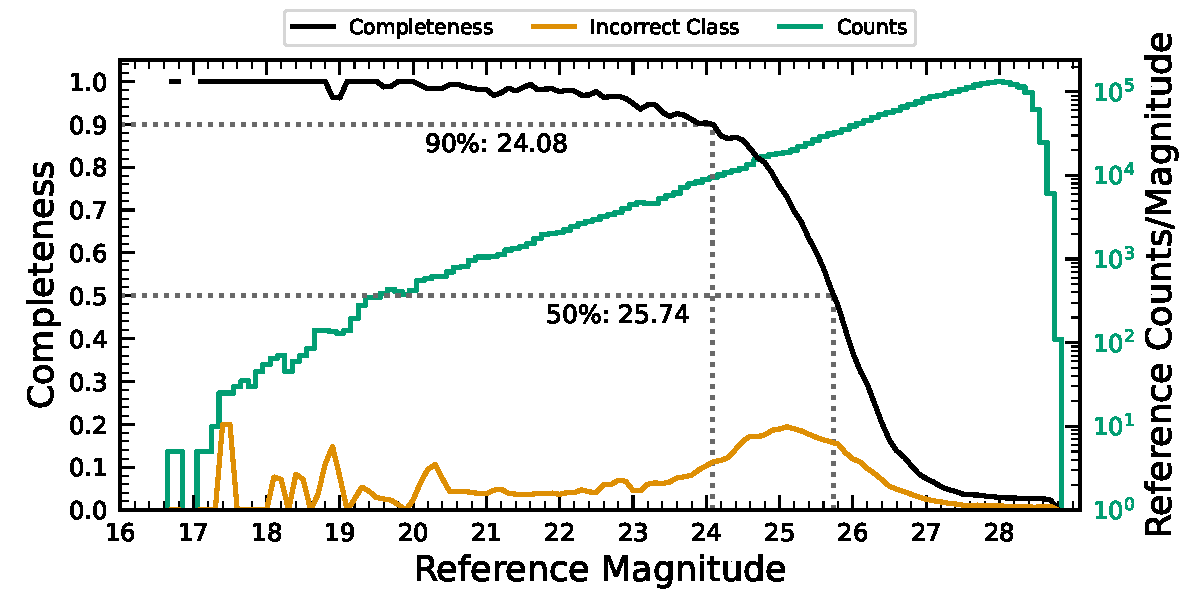
\includegraphics[width=0.98\linewidth]{figures/injected_lsst_cells_v1_5063_i_completeness_any.pdf}
\caption{Completeness as a function of $i$-band CModel magnitude for \gls{DC2}-based injections into a portion of the \gls{ECDFS} field.}
\label{fig:injected_lsst_cells_v1_5063_i_completeness_any}
\vspace{0.1cm}
\end{figure}

\figref{fig:injected_lsst_cells_v1_5063_i_completeness_any} shows completeness as a function of magnitude for these injected objects. The completeness estimates are comparable to results from matching external catalogs. The Hubble Legacy Field catalog \citep{2019ApJS..244...16W,2016arXiv160600841I} reaches 50\% completeness at 26.13\,${\rm mag_{F775W}}$, approximately 0.4 magnitudes fainter; this is roughly equivalent to 25.83\,${\rm mag_{i}}$ from differences in matched object magnitudes. Similarly, completeness drops below 90\% at 23.80${\rm mag_{VIS}}$ matching to Euclid Q1 \citep{2025arXiv250315305E} objects, equivalent to about 23.5\,${\rm mag_{i}}$. 
The Euclid imaging is of comparable or shallower depth, so magnitude limits at lower completeness percentages than 90\% are unreliable, whereas the HST images cover too small and irregular an area to accurately characterize 80-90\% completeness limits.
% DST: Is the above sentence TMI? It can be cut.

At the 80\% completeness limit, nearly 20\% of objects, primarily injected galaxies, are incorrectly classified as stars based on extendedness, which indicates whether a source is more likely to be a point source or an extended source.
Similarly, the fraction of correctly classified injected stars drops to about 50\% at 23.8\,${\rm mag_{i}}$ (90\% completeness).

There are several caveats for this analysis. The selection of objects for matching in any catalog is not trivial. Some fraction of the detections are either artifacts (particularly close to diffraction spikes around bright stars) or otherwise spurious. Additionally, some objects lie in masked regions of one survey but not another, which has not been accounted for. For injected source matching, the reference catalog does not include real on-sky objects. For this reason, we do not quote specific figures for purity; however, based on prior analyses of the \gls{DC2} simulations, purity is generally higher than completeness at any given magnitude.
% DST: The detection curve in DC2 is steeper and fainter than the equivalent source injection curve, despite DC2 having fewer visits. It's unclear whether this is due to (amongst other things) the relative simplicity of artifacts in DC2, differences in assumed filter response/gain, seeing distributions, etc. so this point is probably best left out.

\subsection{Flux Measurement}
\label{ssec:fluxes}

\begin{figure}[htb]
\centering
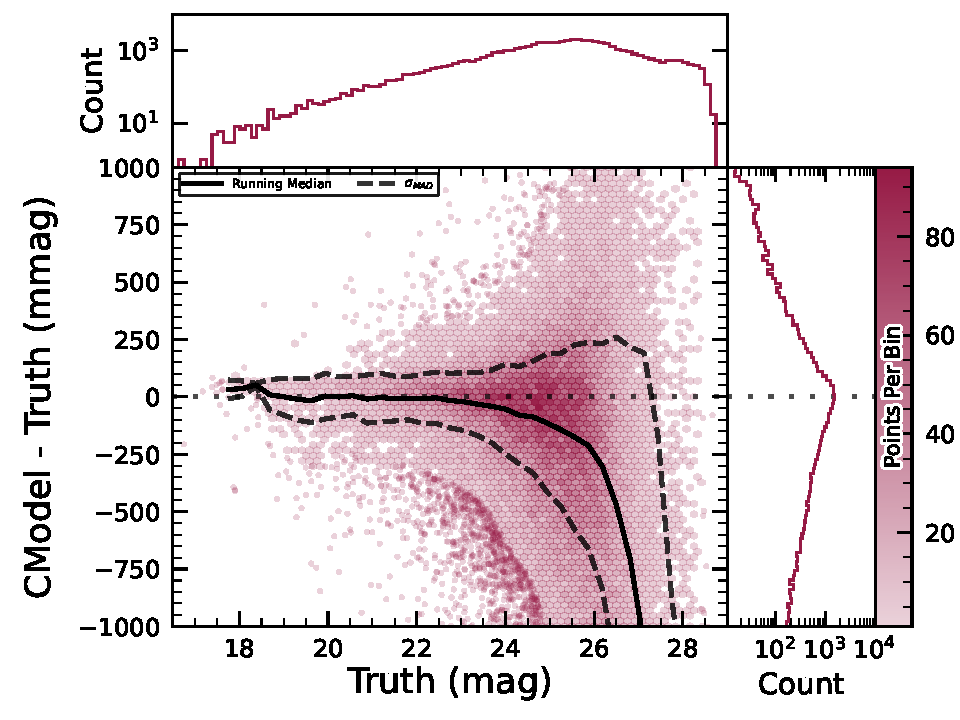
\includegraphics[width=0.98\linewidth]{figures/injected_lsst_cells_v1_5063_i_mag_cmodel.pdf}
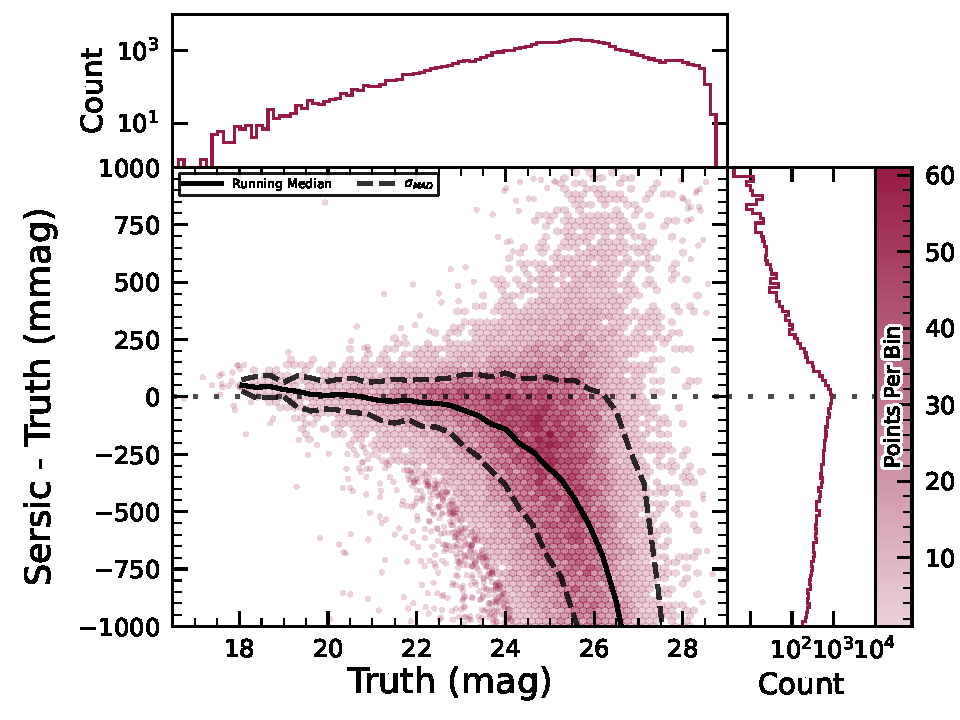
\includegraphics[width=0.98\linewidth]{figures/injected_lsst_cells_v1_5063_i_mag_sersic.pdf}
\caption{Magnitude residuals for matched injected galaxies with the CModel and Sersic algorithms.}
\label{fig:injected_lsst_cells_v1_5063_i_mag}
\vspace{0.1cm}
\end{figure}

\figref{fig:injected_lsst_cells_v1_5063_i_mag} shows $i$-band magnitude residuals for CModel and Sersic measurements using the matched injected galaxies described in \secref{ssec:detection_completeness}.
Similar behavior is seen in other bands.
Sersic fluxes show reduced scatter and are more accurate on average for galaxies brighter than 22.5\,${\rm mag_{i}}$, though CModel's are less biased, with median residuals  slightly closer to zero.
For fainter objects, Sersic fluxes are more biased and less accurate.
The magnitude of this bias is considerably larger than previously seen in simulated data and is being investigated.
Aperture fluxes - including Kron and \gls{GAaP} - are not shown as they are not corrected to yield total fluxes and thus are not recommended for use as total galaxy magnitudes.

\begin{figure}[htb]
\centering
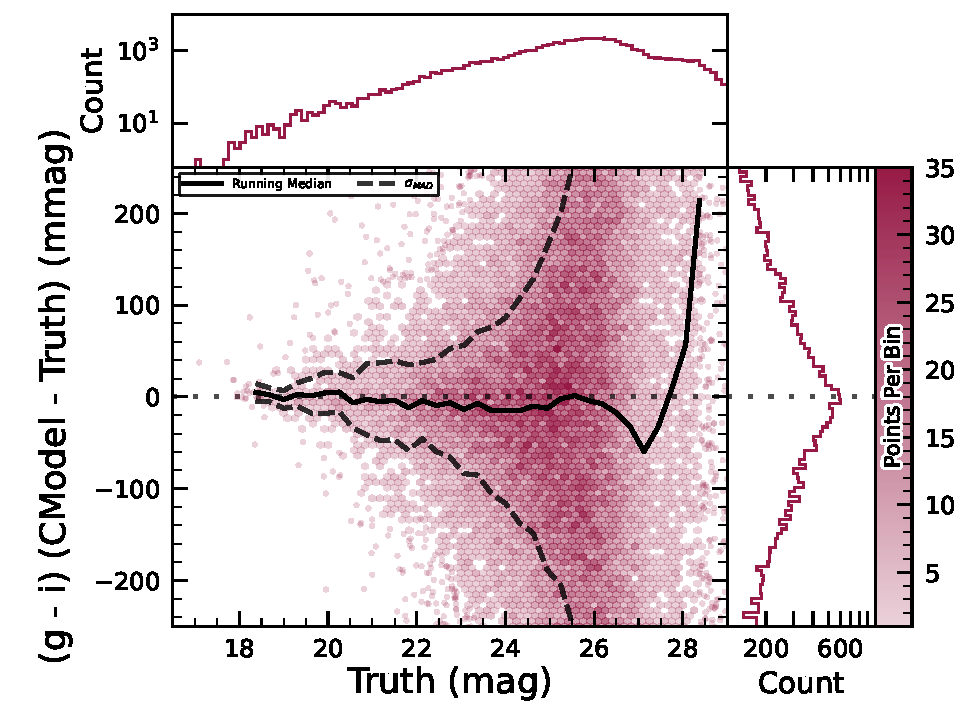
\includegraphics[width=0.98\linewidth]{figures/injected_lsst_cells_v1_5063_r_color_cmodel_g_minus_i.pdf}
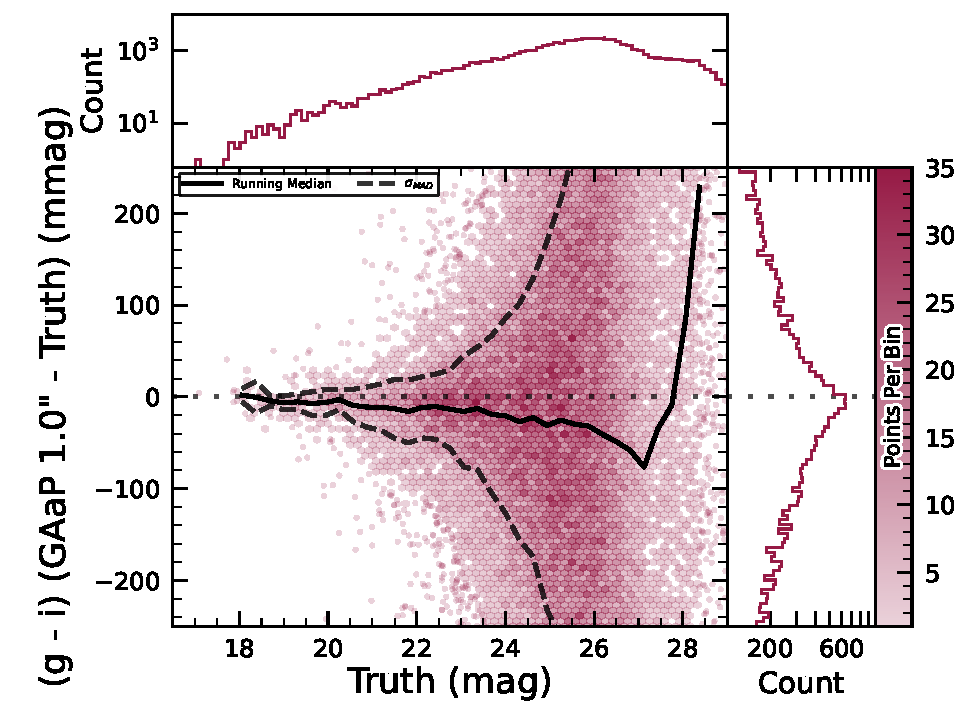
\includegraphics[width=0.98\linewidth]{figures/injected_lsst_cells_v1_5063_r_color_gaap_g_minus_i.pdf}
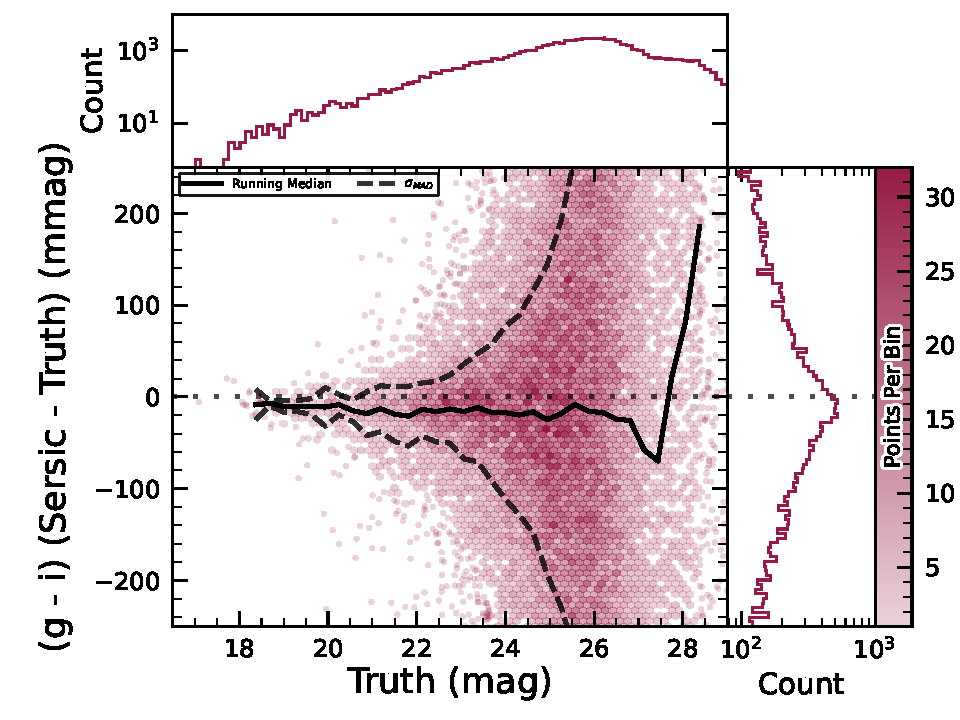
\includegraphics[width=0.98\linewidth]{figures/injected_lsst_cells_v1_5063_r_color_sersic_g_minus_i.pdf}
\caption{$g-i$ color residuals versus injected r-band magnitude for matched galaxies with the CModel, \gls{GAaP} and Sersic algorithms.}
\label{fig:injected_lsst_cells_v1_5063_r_color_g_minus_i}
\vspace{0.1cm}
\end{figure}

\figref{fig:injected_lsst_cells_v1_5063_i_mag} shows $g-i$ color residuals versus $r$-band magnitude for the same sample of galaxies as \figref{fig:injected_lsst_cells_v1_5063_i_mag}.
For this and most other colors, \gls{GAaP} (with a $1''$ aperture) and Sersic colors both yield lower scatter; however, the CModel colors have the smallest bias.
Curiously, the \gls{GAaP} bias appears to be magnitude-dependent, whereas the Sersic bias remains stable from $19<r<26$.
Any of these color measurements are suitable for use for deriving quantities like photometric redshifts, stellar masses, etc.

In addition to photometry, some algorithms include measurements of structural parameters like size, ellipticity, and Sersic index.
One particular known issue is that many (truly) faint objects have significantly overestimated sizes and fluxes, as was also seen in the Dark Energy Survey \citep{2025arXiv250105739B}.
We dub such objects "super-spreaders".
These super-spreaders contribute significantly to overestimated fluxes at the faint end, and are particularly problematic for the Kron algorithm \citep{1980ApJS...43..305K}, which is not recommended for general use.

As mentioned in \secref{ssec:coadd_processing}, the Sersic fits include a free centroid, which is initialized from the fiducial centroid of the object.
Preliminary analyses of matched injected objects suggest that the galaxy \gls{astrometry} residuals are somewhat smaller, and so users of the Sersic photometry should also use these centroid values (if needed).
One caveat is that for faint objects and/or in crowded regions with unreliable deblending, free centroids can drift significantly and potentially towards other objects, so objects with large differences between the fiducial and Sersic \gls{astrometry} should be used with caution.

\subsection{Differential Chromatic Refraction}
%% This is an effect seen in ComCm - this section shows that but no correction is applied to proceessing in DP1.
%% Think we'll need to correct for this in templates  to some degree to prevent dipoles appearing as extrems color sources at hight airmass.
%% Science -- Fed -- measure stellar flar temperatures, AGN uise the effect to identiyf quasar lines - bight emmision lines in quasars as they transiotion.
\label{sec:differential_chromatic_refraction}
\gls{Differential Chromatic Refraction} (DCR) occurs when light passes through Earth’s atmosphere, refracting more for shorter wavelengths, which causes blue light to appear shifted closer to the zenith. 
This wavelength-dependent effect results in the smearing of point sources along the zenith direction, specifically parallel to the parallactic angle. 
The DCR effect is observable in LSSTComCam data, particularly in the angular offset versus g-i band magnitude difference plots,  as shown in \figref{fig:dcr}, which plots all direct sources with \gls{SNR} $>10$ from 41 visits from November 26, 2024. 
When looking at data perpendicular to the parallactic angle, sources show no DCR effect (as expected), forming a clear vertical distribution on the 2-dimensional density plots in \figref{fig:dcr}.

In contrast, sources aligned with the parallactic angle exhibit a tilted, linear distribution, clearly demonstrating the relationship between angular offset and the $g-i$ band magnitude difference, thereby providing a visual indication of the \gls{DCR} effect.

\begin{figure}[htb!]
\centering
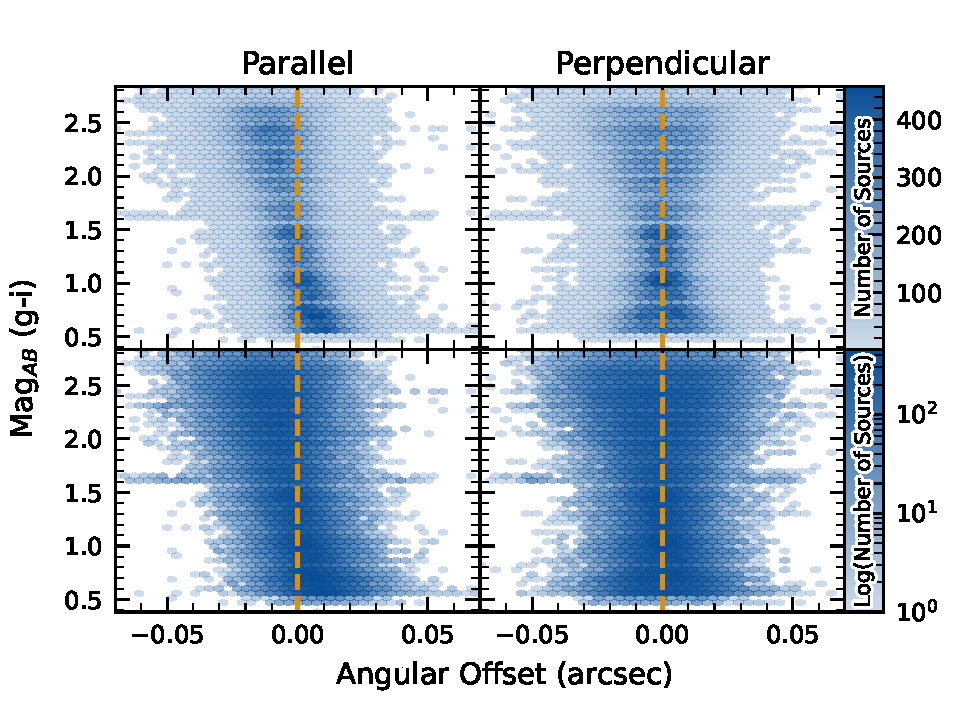
\includegraphics[width=0.98\linewidth]{dcrHexbin.pdf}
\caption{Visualization of \gls{Differential Chromatic Refraction} (DCR) observed in the  LSSTComCam commissioning campaign. The $g-i$ color is computed for every source in the reference catalog that is matched to a direct source in the science image, and the binned density for the full survey is plotted against the angular offset between the reference and detected positions. The angular offset is projected along coordinates parallel and perpendicular to the parallactic angle of the observation, and shows a characteristic correlation along the parallel axis with no correlation along the perpendicular axis. The orange vertical dashed line indicates the expected $g-i$ magnitude distribution at zero angular offset, while the green ‘x’ marks the average $g-i$ magnitude of the plotted sources.}
\label{fig:dcr}
\vspace{0.1cm}
\end{figure}


% Eric
\subsection{Difference Imaging Purity} \label{sec:performance:dia}

We assessed the performance of image differencing using human vetting and source injection (\S \ref{sec:perf:dia_completeness}).
Members of the \gls{DP1} team labeled more than 9500 DIASource image triplets consisting of cutouts from the science, template, and difference images.
We classified these into various real and artifact categories.
The artifact to real ratio was roughly 9:1.
Bright stars are the main source of artifacts.
Correlated noise, primarily in u and g bands, also leads to spurious detections near the threshold.
We expect to be able to mitigate these effects for \gls{LSSTCam}.

Applying a reliability threshold improves the purity of transients but not variable stars; technical limitations at the time of model training prevented injection of variable stars into the synthetic training set.
Reliability models for \gls{LSSTCam} data will be trained on a wider range of input data.

\subsection{Detection Completeness on Difference Images} 
\label{sec:perf:dia_completeness}

We assess the performance of our difference imaging \gls{pipeline} using synthetic source injection on the science images prior to differencing.
We construct a catalog of injected sources by joining two different samples of point sources, a set of hosted sources to emulate transients in galaxies and second set of hostless sources.

The hosts are selected from the \gls{pipeline} source catalog that is produced upstream by imposing a cut in their extendedness measurement, and selecting $N_{\rm src}={\rm min}(100, N\times0.05)$ of the available sources per detector.
%
% filtered_sources = sources[(sources['extendedness'] == 1) & (sources['sizeExtendedness']>0.90) & (sources['calibFlux'] > 0)]
%
For each host we pick a random position angle and radius using its light profile \gls{shape}, and also a random value of brightness for the injected source, with magnitudes higher than the host source.
The hostless sources instead have random positions in the \gls{CCD} focal plane, and with magnitudes chosen from a random uniform distribution with $20 \geq m \geq m_{lim} + 1$  with $m_{lim}$ the limiting magnitude of the image.

We used the \gls{LSST} package \texttt{source\_injection} to include these sources into our test images, we performed a coordinate cross-match task, with a threshold of $0.''5$ to find which of these sources were detected and which were lost, enabling the calculation of a set of performance metrics.
%These include i) the detection completeness as function of signal to noise ratio (S/N), ii) the distribution of the coordinate offsets for the found sources, both in sky coordinates and focal plane coordinates, iii) the flux pull distribution both of PSF photometry measurements as well as aperture measurements, iv) the spatial correlation of the positions of both the found and missed sources, in sky coordinates and focal plane coordinates, v) the magnitude and S/N dependency of the astrometry and photometry recovery for the found sources, vi) the detection efficiency as function of the distance and brightness of the host, and vii) the reliability score of the synthetic sources.
%For all of these listed metrics we find results consistent with our expected parameters and required tolerances.

In \figref{fig:eff_snr_griz} we show the detection completeness as function of the \gls{SNR}, for sources in the \gls{ECDFS} field, for filters \textit{griz}. We observe a completeness $>95\%$ for sources with \gls{SNR}$> 6$, with mean completeness $\simeq 99\%$ and standard deviation of $\simeq 0.7\%$.
%
\begin{figure}[htb!]
\centering
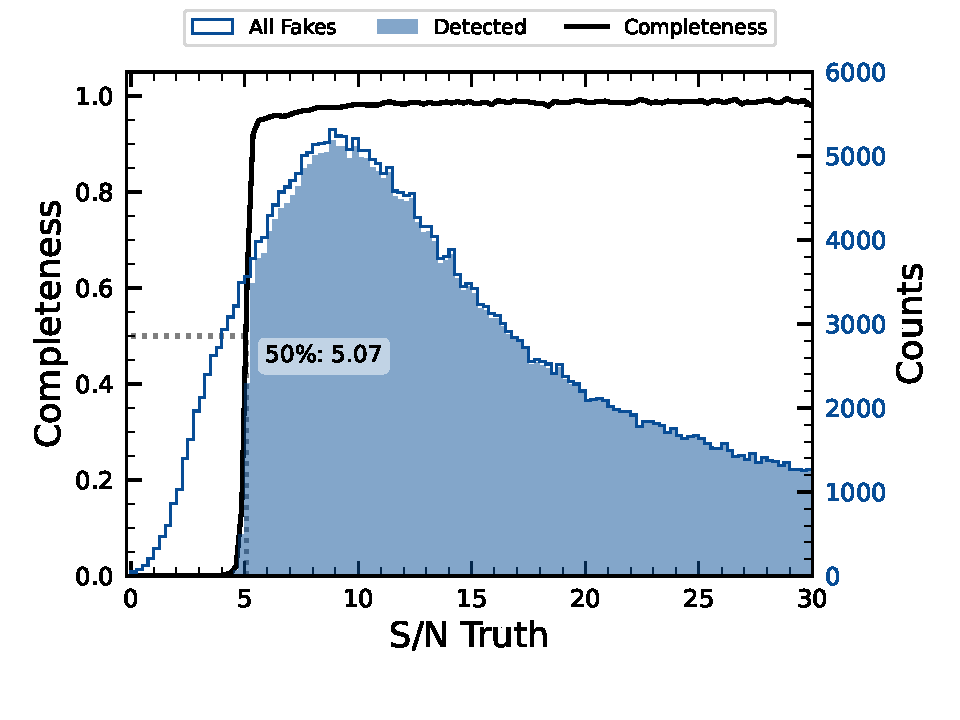
\includegraphics[width=0.98\linewidth]{figures/efficiency_snr_griz.pdf}
\caption{The difference image detection completeness for injected sources in the \gls{ECDFS} field, for filters \textit{griz}, as function of the estimated signal to noise ratio S/N. This completeness is the ratio between the found fake sources (shaded histogram) and all the sources (solid line). The horizontal dashed line represents where the $50\%$ completeness level is reached, at approximately S/N $\simeq 5.07$.}
\label{fig:eff_snr_griz}
\vspace{0.1cm}
\end{figure}
%
In \figref{fig:coordinate_offset_diffim_fakes} we show the distribution of the residuals of the recovered sky coordinates for the detected synthetic sources. The marginal distributions are both centered at zero, and they are compatible with normal distributions $\mathcal{N}(0, 0''.04)$.
%
\begin{figure}[htb!]
\centering
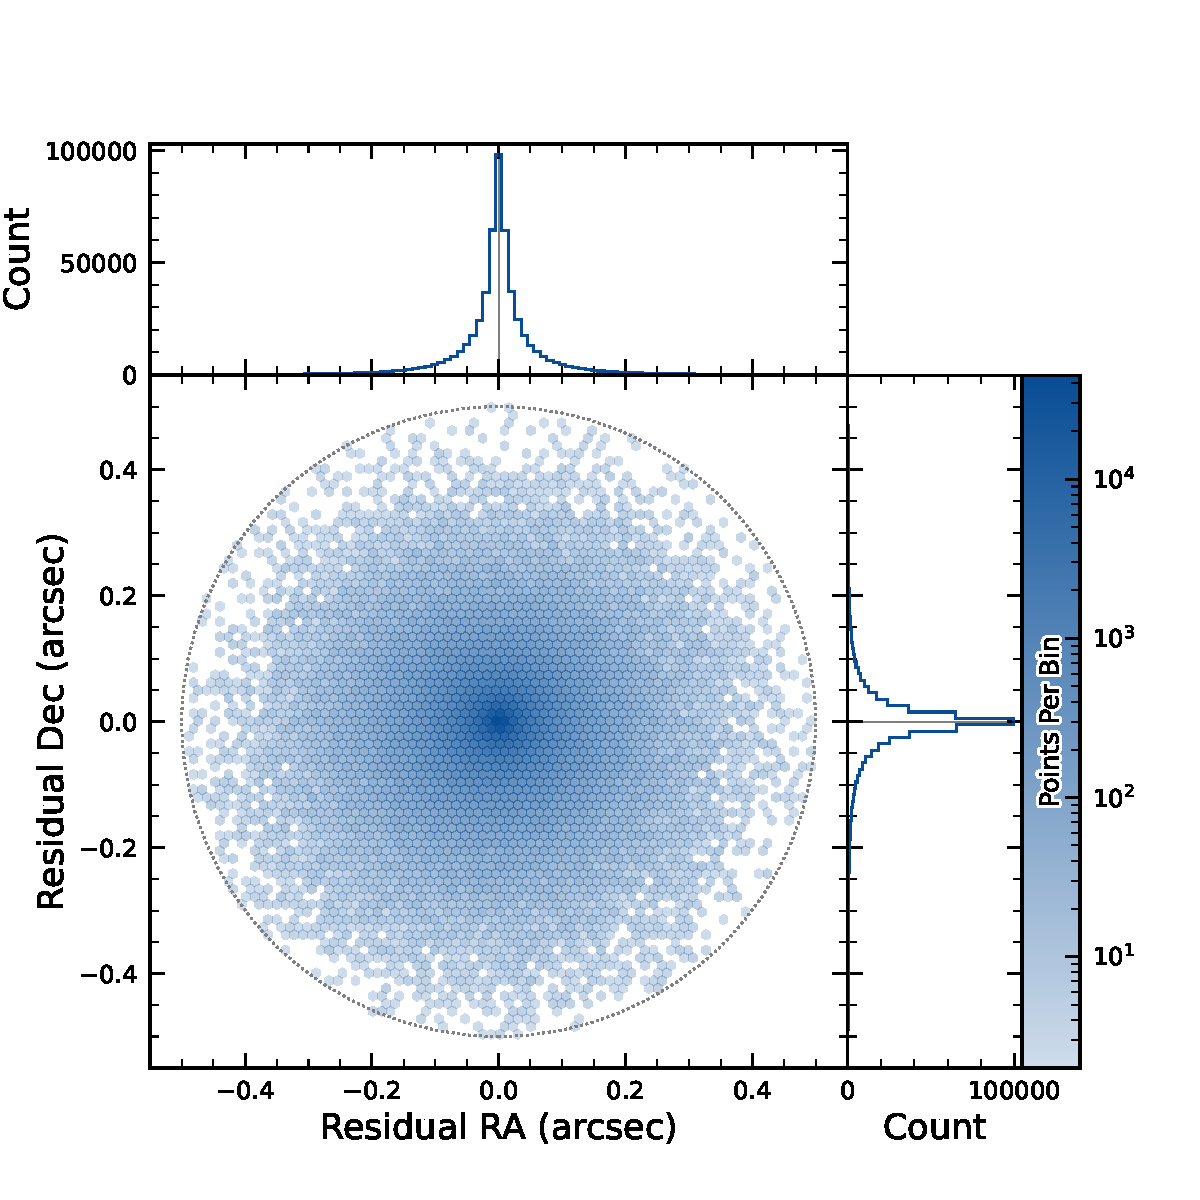
\includegraphics[trim={0 0 0 0},width=\linewidth]{figures/coordinate_offsets_hexbin.pdf}
\caption{Coordinate residuals for detected synthetic sources in difference images, between recovered and true position of the sources in the \gls{ECDFS} field. In the top and right panels we include the histogram of these offsets. The circle reflects the matching radius of $0''.5$.}
\label{fig:coordinate_offset_diffim_fakes}
\end{figure}
%
In \figref{fig:phot_residual_diffim_fakes} we show the recovered magnitudes for our detected synthetic sources in the \textit{i} filter, using \gls{PSF} photometry on the difference images, and also show marginal distributions of the true magnitudes for fake sources, and the residuals on the left, split into hosted and hostless.
%
Our \gls{flux} measurements are accurate within a wide range of magnitudes, for both hosted and hostless synthetic sources. 
For true $m_i < 22.2$, the median PSF magnitudes residuals are $<0.1$. 
When considering the \gls{flux} pulls $\delta = (f-f_{\rm{True}})/\sigma_f$ for PSF \gls{flux} $f$ and error $\sigma_f$, we find that $|\left<\delta\right>| <0.1$, and $\sigma_\delta < 1.1$ for $m_i<21.6$.
%
\begin{figure}
    \centering
    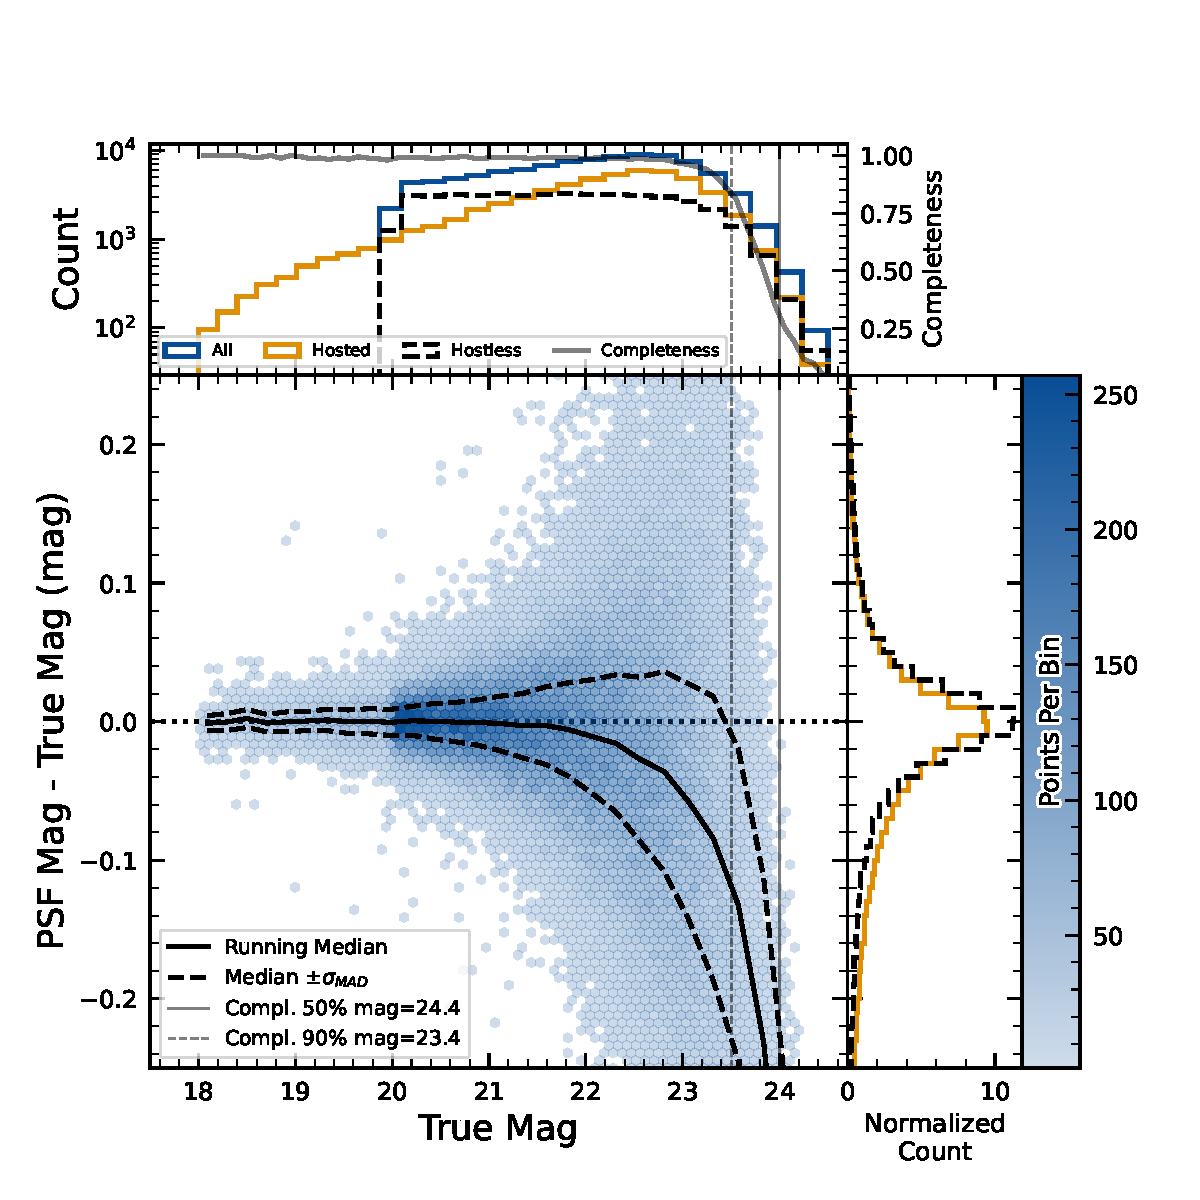
\includegraphics[width=\linewidth]{figures/hexbin_psf_mag.pdf}
    \caption{Magnitude residuals for \gls{PSF} photometry on difference images for ECDFS field in $i$ for detected fake sources. In black solid and dashed lines: the running median, and the mean absolute deviation. Top panel: the distribution of true magnitudes for hostless and hosted fakes sources. Right panel: the distribution of magnitude residuals for hostless and hosted sources.}
    \label{fig:phot_residual_diffim_fakes}
\end{figure}

% Jake/Mario
\subsection{Solar System}
\label{sec:performance:solsys}

\subsubsection{Asteroid Linking Performance}

\gls{DP1} performance evaluation of asteroid linking focused on demonstrating discovery capability.
The solar system discovery \gls{pipeline} produced 269,581 tracklets, 5,691 linkages, and 281 post-processed candidates.

We performed a conservative manual investigation of these 281 candidates, producing a curated list of \nnewasteroiddiscoveries probable new asteroid discoveries.
All of these candidates are identified as main-belt asteroids.
As described in Section~\ref{sec:drp:solsys}, post processing of the {\tt heliolinc} output with {\tt link\_purify} produced a final set of 281 candidate linkages, ranked with the most promising candidates first.
Using {\tt find\_orb} \citep{findorb}, we derived orbit fits for each candidate, sorting the resulting list by $\chi_{\rm dof}^2$, the quality of the fit.
Manual inspection of the linkages indicated that those ranked 0--137 corresponded to unique real asteroids; ranks 138--200 contained additional real objects intermixed with some spurious linkages; an d ranks higher than 200 were essentially all spurious.
This analysis indicates that it will be possible to identify cuts on quality metrics like $\chi^2$ to derive discovery candidate samples with high purity; determining the exact quantitative cut values requires more data with \gls{LSSTCam}.
We next removed all observations matched to known asteroids (using \gls{MPC}'s MPChecker service), reducing the number of candidates to 97.
Of these, four had strong astrometric and/or photometric outliers, likely due to self-subtraction in difference images due to the unavoidable limitations of template generation from the limited quantity of data available from  \gls{LSSTComCam}.
We suspect these four linkages do correspond to real objects, but have chosen to discard them out of an abundance of caution.
The remaining \nnewasteroiddiscoveries were submitted to the Minor Planet Center and accepted as new discoveries, demonstrating the \gls{LSST} pipelines are able to successfully discover new solar system objects.
%\jake{We should cite the MPEC with discoveries, once we do submit and the MPEC becomes available}

\subsubsection{Asteroid Association Performance}

Solar system association associated \nsolarsystemsources DiaSources to \nsolarsystemobjects unique solar system objects. 
%\jake{Update this after table update!}
These include 3,934 DiaSources to 338 already-known \gls{MPC} objects and 2,054 DiaSources to the \nnewasteroiddiscoveries  newly-discovered objects.
Association also picked up an additional 143 detections of newly discovered objects.
% \jake{This too - new parameter in notebook.}
These were not originally found by the discovery pipelines as they didn't satisfy the number and/or maximum time span requirements to form tracklets.

\begin{figure}[htb!]
\centering
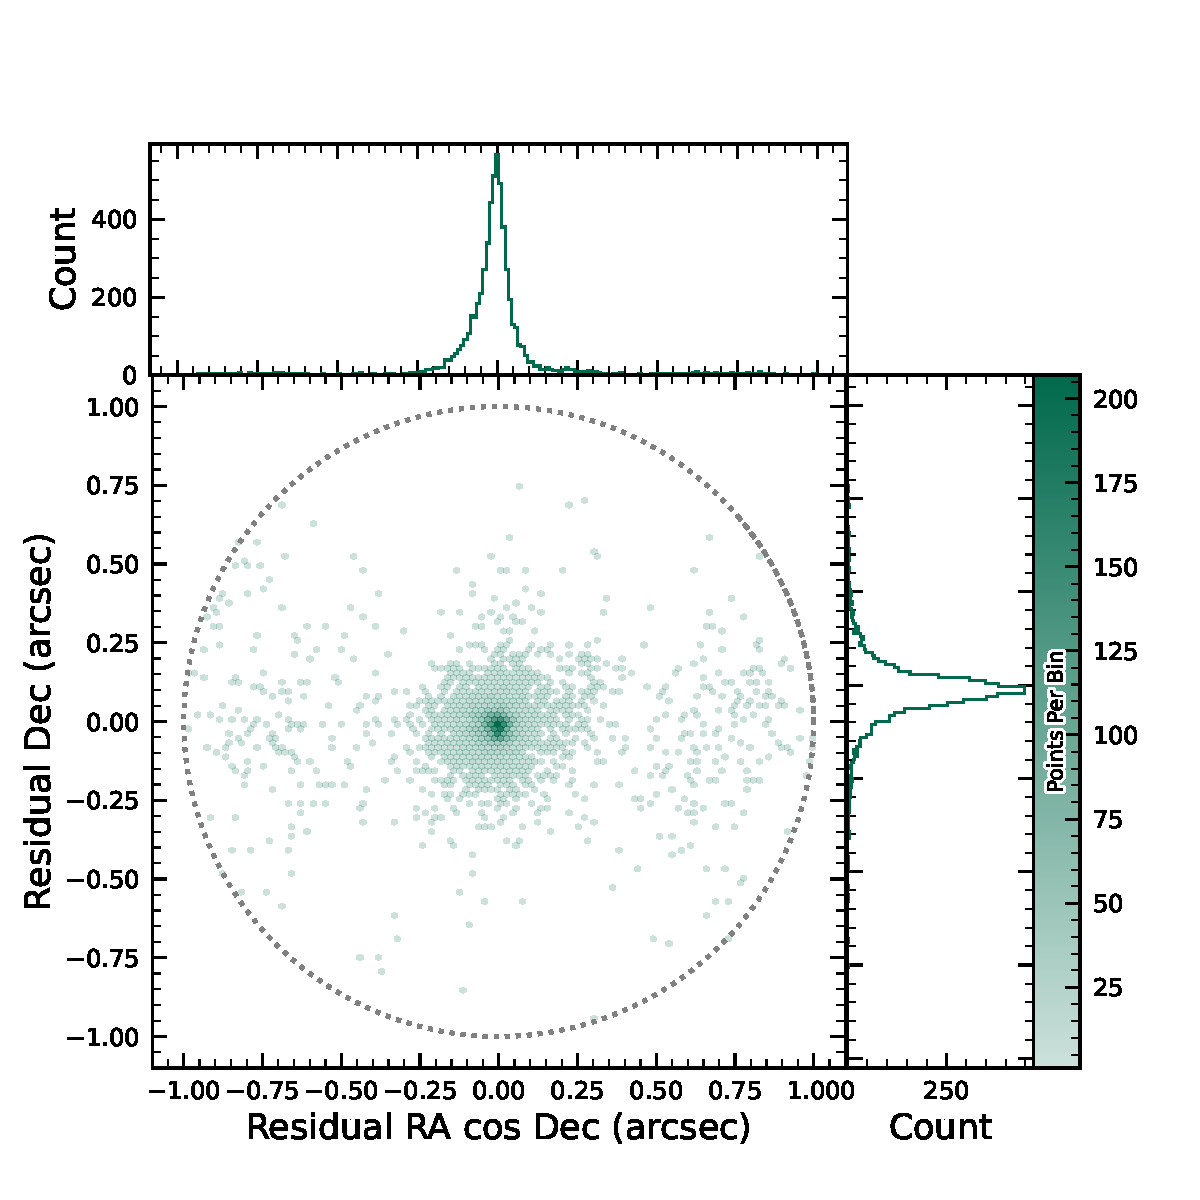
\includegraphics[width=0.98\linewidth]{figures/sso_residuals.pdf}
\caption{Astrometric residuals between expected and observed positions of SSOs in \gls{DP1}. The median residuals are $0.''001$ and $-0.''016$ in R.A./Dec direction, with the standard deviations of $0.''19$ and $0.''10$, respectively. No detectable detectable systematic offset from zero indicates there are no major errors in either timing or astrometry delivered by the Rubin system. The wider scatter in the RA-direction is due to objects whose measured orbital elements are less well constrained, translating to larger along-track positional errors in the predicted positions.}
\label{fig:sso_residuals}
\vspace{0.1cm}
\end{figure}

The astrometric residuals of known asteroid association are shown in Figure \ref{fig:sso_residuals}. 
%\jake{Todo:} 
Astrometric precision for solar system sources is excellent, the majority of objects detected within $0''.1$ of their expected positions. 
Taking the unsigned median residuals to search for biases, we find that previously-known objects have mean residuals of $0.''001$ and $-0.''016$ in the \gls{RA} and Dec directions respectively, while newly-discovered objects have mean residuals of $-0.''035$ and $-0.''010$ in the \gls{RA} and Dec directions, respectively. 
These mean residuals are small enough to eliminate the possibility of a timing offset greater than the second-scale shutter motion (which is uncharacterized for LSSTComCam).

\subsection{Crowded Fields}
Two of the seven \gls{DP1} target fields exhibit high stellar density, 47 Tucanae and the Fornax dwarf galaxy.
47 Tucanae was chosen as an initial stress test for the science pipelines processing.
The Fornax dwarf galaxy also exhibits high stellar density, particularly in its central regions.
%\yusra{Explain where the pipelines broke down. and  how the performance is different in the 2 crowded fields}
